\subsection{Implementation of \texttt{mm\_malloc}}

In order to make the concepts used in \code{mm_malloc} clearer, I will first explain how the dynamic memory allocator is laid out.

\subsubsection{Memory layout of my dynamic memory allocator}

My dynamic memory allocator uses the notion of blocks in the heap that are either allocated or free. To manage free blocks, I use an explicit free list, which will be described later.

Each block is 8-byte (double word) aligned and consists of a header, footer, and payload. Each block is laid out in memory as shown on \autoref{fig:block-layout} below.

\begin{figure}[H]
  \centering
  \hbox{\makebox[\textwidth][c]{
    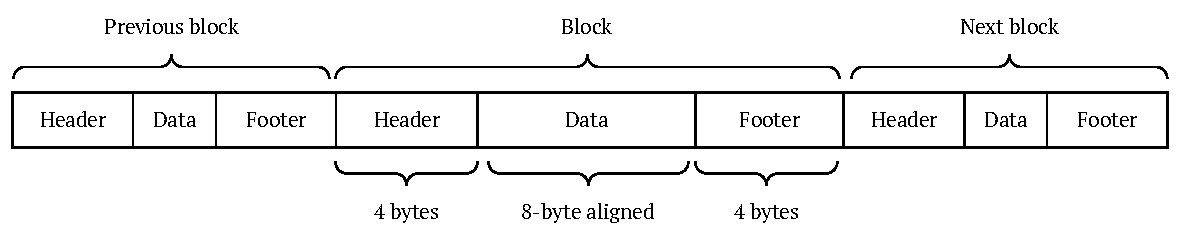
\includegraphics[scale=0.95]{figures/block-layout-example.pdf}
  }}
  \caption{The layout of blocks in memory for my dynamic memory allocator. ``Data'' is used synonymously with ``payload''.}
  \label{fig:block-layout}
\end{figure}

The header consists of the block's size and a flag that indicates if the block is allocated or free. This is all packed into a 32-bit integer. The size of the block is always a multiple of 8, meaning the least significant bit is always 0. Therefore, we can use this single bit to store the allocation flag.

The footer is a duplicate of the header, but it only exists for free blocks.

When we obtain a pointer to a block, the pointer points to the first byte of the payload, not the header.

For allocated blocks, the payload is where the user's data is written to. But for free blocks, because we are using an explicit free list, we use two words (8 bytes) in the payload to store two 4-byte pointers to the next and previous free blocks.

In order to avoid fragmentation, adjacent free blocks are joined every time a block is freed, or if the heap is extended. This means that the blocks in memory are not guaranteed to remain statically laid out - their sizes can change.

\subsubsection{Components of my \code{mm_malloc} function}

The most important parts of my \code{mm_malloc} implementation (which will all be described in the next sections) are:

\begin{enumerate}
  \item Finding a free block
  \item Optionally extending the heap
  \item Coalescing blocks
  \item Manipulating the free list
  \item Marking a block as allocated
  \item Splitting existing blocks
\end{enumerate}

\subsubsection{The explicit free list}

It's possible to find a free block on the heap by iterating over all blocks. However, this takes $O(b)$ time (with $b$ being the amount of blocks). Instead, I've implemented an explicit free list, which uses the payload to store pointers to the next and previous free blocks. Using this is a doubly linked list, it's possible to iterate through only the free blocks on the heap, skipping all already-allocated blocks. The structure of free blocks in my implementation is illustrated on \autoref{fig:free-list-structure}.

\begin{figure}[H]
  \centering
  \hbox{\makebox[\textwidth][c]{
    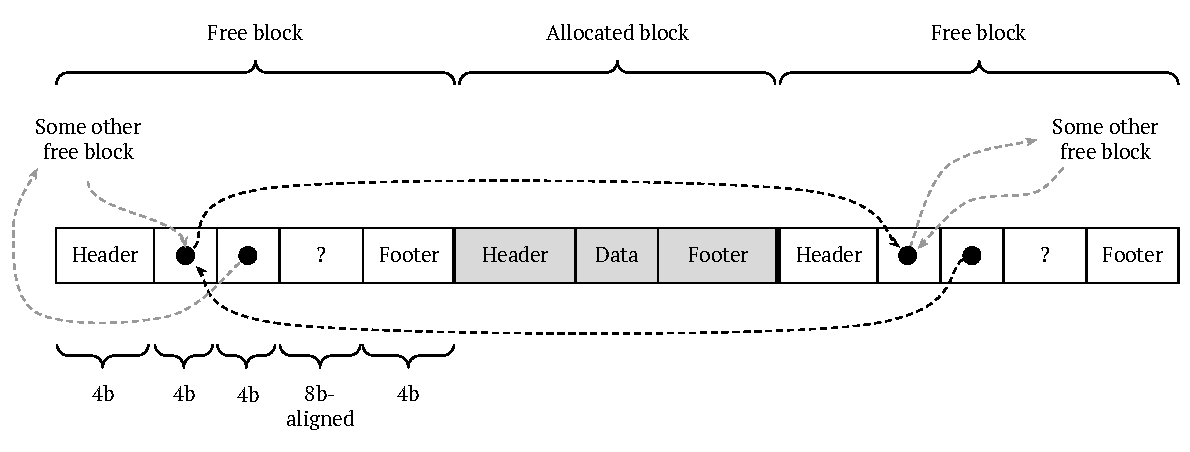
\includegraphics[scale=0.90]{figures/free-list-layout-example.pdf}
  }}
  \caption{An illustration of free blocks in my memory allocator. A block still has a header and footer, but it now also uses the first 8 bytes to store two 4-byte pointers to the next and previous free blocks, respectively. When there is no next or previous free block, the pointer is null. The \code{?} indicates that the rest of the data in a free block is just garbage.}
  \label{fig:free-list-structure}
\end{figure}

With this, it only takes $O(f)$ time (with $f$ being the amount of free blocks) in the worst case to find a free block large enough, if any such block exists.
